\section{Scaling With the Lane Count}\label{sup:lanes}
\begin{figure}[t]
\centering
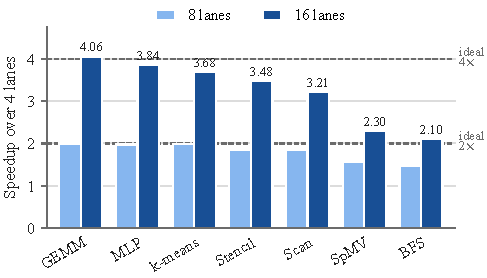
\includegraphics[width=\columnwidth]{lanes_speedup.pdf}
\caption{Speedup of each application at 8 and 16 lanes over a four-lane SIMTiX,
with four warps and a 16~KiB L1 whose line is one word per lane. Dashed lines mark
linear speedup.}
\label{fig:lanes}
\end{figure}

The lane count $L$ is a parameter: it sets the warp width, the line of the memory
engine and the L1 (one word per lane, with the L1 kept at 16~KiB) and the burst
length of the AXI4 master. Fig.~\ref{fig:lanes} shows the speedup over four lanes,
with four warps throughout; all seven applications pass their bit-exact checks at
every lane count. From eight to 16 lanes GEMM gains $2.03\times$, the MLP
$1.95\times$, the stencil $1.88\times$ and k-means $1.86\times$, while scan gains
$1.74\times$, SpMV $1.47\times$ and BFS $1.43\times$. GEMM, the stencil, k-means
and the MLP keep every lane active, and the scan 95\% of them. SpMV and BFS diverge
on their row and neighbor loops, where a warp runs until its longest row or
adjacency list ends, and their lane utilization falls from 66\% and 55\% at four
lanes to 59\% and 43\% at eight and 57\% and 34\% at 16. Their gathers also touch
about one line per lane, and the memory engine sends one request per line: from
eight to 16 lanes the warp instructions of SpMV halve, but its L1 accesses fall
only from 12,100 to 9,625, and its IPC drops from 0.43 to 0.33.

The cost grows faster than the lane count. Four lanes use 43,119 LUTs at
113.5~MHz and eight lanes 84,443 at 101.6~MHz. Placed, the 16-lane design
occupies 190,401 LUTs, 83\% of the XCZU7EV and 2.3 times the eight-lane design,
and 96\% of the device's configurable logic blocks hold some of its logic. Each lane's FPU stays at 4.8k LUTs, but the memory engine,
implemented alone in its board configuration, grows from 4,645 LUTs at four lanes
to 12,576 at eight and 42,474 at 16, by 2.7 and then 3.4 times per doubling; all
three meet 100~MHz. The engine selects the word of every lane from a line that
itself holds one word per lane, places every lane's store data into that line,
and, for the aggregated AMOs, compares the word addresses of every pair of lanes.
These structures grow with the square of the lane count. Wider warps are
therefore limited by the memory engine rather than by the lanes, and beyond eight
lanes more cores, or an engine that serves part of a warp per cycle, are the
better way to add throughput.

The 16-lane run also exposed the stack bound of Section~\ref{P-sec:arch}. Our stack
had eight frames, which by the bound suffices for eight lanes. In SpMV at 16
lanes, a warp whose rows have more than eight different lengths leaves its loop at
more than eight different iterations, pushing a frame each time, and overflowed
the stack. Sizing the stack by the lane count removed the failure; at eight lanes
the design is unchanged.
